\documentclass[a4paper, 11pt]{article}
\usepackage[top=2cm, bottom=2cm, left=1.5cm, right=1.5cm]{geometry}
\usepackage[utf8]{inputenc}
\usepackage{amsmath, amsfonts, amssymb}
\usepackage{graphicx}
\usepackage[brazil]{babel}


\begin{document}

\begin{center}
\textbf{Liste de Números Complexos}
\end{center}

\textbf{ \underline{Resumo} }
\\


\begin{itemize}

\item $\mathbb{R} \longrightarrow$ \textbf{Reta} Real

\item $\mathbb{C} \longrightarrow$ \textbf{Plano} Complexo (também chamado de Plano de Argand-Gauss)

\item $ \mathbb{C} = \{ z = a + bi \, | \, a,b \, \in \mathbb{R} \textrm{, onde } i^2 = -1 \} $

\item A representação de um complexo como um ponto no plano recebe o nome de \textbf{afixo}

\item Multiplicar por $i$ corresponde a rotacionar um complexo exatamente $90^{\circ}$ no sentido anti-horário, mantendo o tamanho original do vetor. Para rotacionar por ângulos diferentes, bem como para mudar o módulo, multiplicaremos por números complexos específicos, dependendo de cada resultado que se queira obter.

\item Para converter de graus para radianos (ou vice-versa), faça a seguinte regra de três:

$\dfrac{\theta}{\alpha^{\circ}} = \dfrac{\pi}{180^{\circ}}$ , com $\theta$ em radianos

\item Forma algébrica (ou retangular)


	\begin{itemize}

\item $ \textrm{Parte Real e Parte Imagin\'aria: } a = \textrm{Re} (z) \textrm{ e } b = \textrm{Im} (z)$ representam as coordenadas do complexo no plano $\longrightarrow z = (a,b)$

\item $ \textrm{Igualdade: } z_1 = z_2 \longleftrightarrow a + bi = c + di \longrightarrow a = c \textrm{ e } b = d $

\item $ \textrm{Soma: } z_1 + z_2 = (a + bi) + (c + di) = (a + c) + (b + d)i \in \mathbb{C} $

\item $ \textrm{Multiplicação: } z_1 \cdot z_2 = (a + bi) \cdot (c + di) = (ac - bd) + (bc + ad)i \in \mathbb{C}$

\item $ \textrm{Conjugado: } z = a + bi \longrightarrow \overline{z} = a - bi $

\item $ \textrm{Divisão: } \dfrac{z_1}{z_2} = \dfrac{ z_1 \cdot \overline{z_2} }{z_2 \cdot \overline{z_2}} $

	\end{itemize}

\item Forma trigonométrica (ou polar)


	\begin{itemize}
	
\item Módulo: $ |z| $ é o tamanho do vetor que liga a origem até o afixo, no plano complexo	

\item Argumento: $ arg(z) = \theta $; ângulo entre a parte positiva do eixo dos reais, seguindo em sentido anti-horário, até o vetor que representa o número complexo
	
\item Notação: $ z = |z|cis(\theta) = (\, |z| ; arg(z) \,)$

\item Soma: \textbf{não faça somas nessa forma, porque é muito complicado e trabalhoso}

\item Multiplicação: $z_1 \cdot z_2 = |z_1| \cdot |z_2| \cdot cis(\theta_1 + \theta_2) $

\item Conjugado: $z = |z| \cdot cis(\theta) \longrightarrow \overline{z} = |z| \cdot cis (-\theta) $

\item Divisão: $ \dfrac{z_1}{z_2} = \dfrac{|z_1|}{|z_2|} \cdot cis(\theta_1 - \theta_2) $

	\end{itemize}


\item Conversão: algébrica $\longleftrightarrow$ trigonométrica


	\begin{itemize}
	
\item Algébrica $\longrightarrow$ trigonométrica

$ |z| = \sqrt{a^2 + b^2} $ e $ arg(z) = arctan (\dfrac{b}{a}) $

\item Trigonométrica $\longrightarrow$ algébrica

$ a = |z| \cdot cos(\theta) $ e $ b = |z| \cdot sin(\theta) $
\\
\\
	
	\end{itemize}


\item Fórmulas de De Moivre

	\begin{itemize}

\item As fórmulas de De Moivre falam de potenciação e radiciação com $n \in \mathbb{Z}$. Portanto, a menos que você fique confortável calculando coisas do tipo $z^n = (a + bi)^n$, expandindo o Binômio de Newton, ou coisas do tipo $\sqrt[n]{z} = \sqrt[n]{a + bi}$, sugiro que use sempre a forma trigonométrica para calculá-las.

\item $n \in \mathbb{Z}$

\item Potenciação: $ z^n = |z|^n \cdot cis(n\cdot\theta)$

\item Radiciação: $ \sqrt[n]{z} = \sqrt[n]{|z|} \cdot cis( \dfrac{\theta + 2k\pi}{n} ) $
\\
	\end{itemize}
\end{itemize}


\begin{center}
\textbf{\underline{EXERCÍCIOS}}
\end{center}


\begin{enumerate}

\item  Segundo o matemático Leopold Kronecker (1823-1891), Deus fez os números inteiros, o resto é trabalho do homem. Os conjuntos numéricos são, como afirma o matemático, uma das grandes invenções humanas. Assim, em relação aos elementos desses conjuntos, é correto afirmar que:

(a) o produto de dois números irracionais é sempre um número irracional.

(b) a soma de dois números irracionais é sempre um número irracional.

(c) entre os números reais 3 e 4, existe apenas um número irracional.

(d) entre dois números racionais distintos existe pelo menos um número racional.

(e) a diferença entre dois números inteiros negativos é sempre um número inteiro negativo.


\item Seja y um número real compreendido entre $\dfrac{1}{4}$ e $\dfrac{1}{2}$. Qualquer que seja o valor de y, ele pertencerá ao conjunto
	\begin{enumerate}
	\item $ \{ x \in \mathbb{Z} \, | \, x \leq \,1 \} $
	\item $ \{ x \in \mathbb{R} \, | \, \dfrac{1}{4} < x < \, \dfrac{1}{2} \} $
	\item $ \{ x \in \mathbb{Q} \, | \, -1 < x \leq \, 2 \} $
	\item $ \{ x \in \mathbb{I} \, | \, x < \, \dfrac{1}{2} \} $
	\item $ \{ x \in \mathbb{N} \, | \, x \geq  \, \dfrac{1}{2} \} $
	\end{enumerate}


\item Classifique em verdadeiro ou falso os itens a seguir:
	\begin{enumerate}
	\item $\mathbb{R} \subset \mathbb{C}$
	\item $\mathbb{C} \subset \mathbb{R}$
	\item $\mathbb{N} \subset \mathbb{C}$
	\item $\mathbb{Q} \cup \mathbb{I} \subset \mathbb{C}$
	\item $\mathbb{Q} \cup \mathbb{I} \subset \mathbb{R}$
	\item $\mathbb{Q} \cup \mathbb{I} \supset \mathbb{R}$	
	\end{enumerate}

\item Marque a(s) proposição(ões) VERDADEIRA(S), em relação aos conjuntos numéricos $\mathbb{N}, \mathbb{Z}, \mathbb{Q}, \mathbb{R} \textrm{ e } \mathbb{C} $

(a) A soma de três números ímpares consecutivos é $159$. O maior dos três é $55$.

(b) Se $x$ e $y$ são números racionais, então $x+y$ e $x \cdot y$ também são racionais.

(c) Dado um número complexo qualquer $x = a+bi$, existe sempre um número complexo $y$ tal que $x \cdot y$ é real.

(d) Se x é um número negativo, então $\sqrt{x}$ não existe.

(e) A forma trigonométrica do número complexo $3\sqrt{3} + 3i$ é o número $6\cdot cis (\dfrac{\pi}{6})$ 

\item Identifique as partes real e imaginária dos números a seguir
	\begin{enumerate}
	\item $z = \dfrac{1}{3} + i$
	\item $z = -3 - 27i$
	\item $z = 2019$
	\item $z = -i$
	\end{enumerate}

\item \textbf{Desafio 1:} O que significa afirmar sobre os conjuntos $\mathbb{A}$ e $\mathbb{B}$ que $\mathbb{A} \subset \mathbb{B}$ e $\mathbb{B} \subset \mathbb{A}$?
\\

%%%%%%%%%%%%%%%%%%%%%%%%%%%%%%%%%%%%%%%%%%%%%%%%%%%%%%%%%%%%%%%%%%%%%%%%%%%%%%%%%

\begin{center}
	\textbf{Forma algébrica (ou retangular)}
	\\
\end{center}


\item Represente geometricamente os complexos:
	\begin{enumerate}
	\item $z = 1 + i$
	\item $z = -2i$
	\item $z = 4i$
	\item $z = -5$
	\item $z = 4 - i$
	\item $z = 3 + 2i$
	\end{enumerate}

\item Sejam os complexos $v = (-2,x)$ e $w = (y,-3)$.
	\begin{enumerate}
	\item Escreva $v$ e $w$ na forma algébrica convencional.
	\item Determine $x$ e $y$ reais tais que $v + w = -4 + 2i$ 
	\end{enumerate}

\item Determine $p \in \mathbb{R}$ de modo que $z = (1-p)+(p^2-1)\cdot i$ seja um número real não nulo.

\item Calcule o valor real de $x$ tal que: $(x^2 - 9) + (x + 3)i = 0$

\item Mostre que, para todo $z \in \mathbb{C}, \, \overline{\overline{z}} = z$.

\item Determine a fórma algébrica dos seguintes quocientes:
	\begin{enumerate}
	\item $\dfrac{6 - 2i}{4 + 2i}$
	\item $\dfrac{5i}{3-4i}$
	\item $\dfrac{4 + i}{4 - i}$
	\item $\dfrac{6}{5i}$
	\item $\dfrac{2i}{1-i}$	
	\item $\dfrac{12-i}{7+8i}$	
	\end{enumerate}

\item Determine os números reais $m$ e $n$ para que as igualdades sejam verdadeiras:
	\begin{enumerate}
	\item $m+(n-1)i = -4+3i$
	\item $(n-2,m+5) = (3,-2)$
	\item $(m-3)+(n-2)i = 5i$
	\item $(m-n+1)+(2m+n-4)i = 0$
	\end{enumerate}

\item Sendo i a unidade imaginária pergunta-se: quantos números reais $a$ existem para os quais $(a+i)^4$ é um número real?

\item Utilize o conjugado $\overline{z}$ para obter a expressão para $z^{-1}$, com $z \neq 0$.

\item Mostre algebricamente a validade das propriedades a seguir:
	\begin{enumerate}
	\item $z \cdot \overline{z} = |z|^2$
	\item $|z_1 \cdot z_2| = |z_1| \cdot |z_2|$
	\item $|\dfrac{z_1}{z_2}| = \dfrac{|z_1|}{|z_2|}$, em que $z_2 \neq 0$
	\end{enumerate}

\item \textbf{Desafio 2:} Você se lembra de que o produto notável $(x + y) (x - y)$ representa uma fatoração possível para $x^2 - y^2$? Com base nisso e nos conhecimentos que obteve, exiba uma possível fatoração para $x^2 + y^2$. 

\item \textbf{Desafio 3:} Dado um número complexo $z = x + iy$, o seu conjugado é o número $\overline{z} = x - iy$.
	\begin{enumerate}
	\item Resolva as equações: $z \cdot \overline{z} = 4$ e $z^2 = \overline{z}^2$
	\item Ache os pontos de intersecção dos lugares geométricos que representam as soluções dessas equações.	
	\end{enumerate}


%%%%%%%%%%%%%%%%%%%%%%%%%%%%%%%%%%%%%%%%%%%%%%%%%%%%%%%%%%%%%%%%%%%%%%%%%%%%%%%
\begin{center}
	\textbf{Forma trigonométrica (ou polar)}
	\\
\end{center}


\item Determine o módulo e argumento principal dos números complexos dados:
	\begin{enumerate}
	\item $z_1 = 4 + 4i$
	\item $z_2 = -5i$
	\item $z_3 = -\sqrt{3} + i$
	\item $z_4 = - \dfrac{1}{3} - \dfrac{1}{3}i$
	\end{enumerate}

\item Determine a fórmula polar dos complexos $x$ e $y$ que satisfazem o sistema
\\
	
	$\left\{ \begin{array}{c}
	2xi+y = -3+i\\
	x+yi = -1\\
	\end{array}
	\right.$
	\\

\item Escreva os seguintes complexos na forma trigonométrica:
	\begin{enumerate}
	\item $z = - \dfrac{5\sqrt{3}}{2} + \dfrac{5}{2}i$
	\item $z = 2i$
	\item $z = \dfrac{1}{2} + \dfrac{\sqrt{3}}{2}i$
	\item $z = (1 - i)^2$
	\end{enumerate}

\item Sabendo que $z_1 = 4\cdot(cos120^{\circ} + i\cdot sin120^{\circ})$ e que $z_1\cdot z_2 = 2\cdot(cos270^{\circ} + i\cdot sin270^{\circ})$, determine:
	\begin{enumerate}
	\item a forma polar de $z_2$
	\item a forma algébrica de $z_2$
	\end{enumerate}

\item São dados os números complexos:

$z_1 = 6\cdot(cos240^{\circ} + i\cdot sin240^{\circ})$

$z_2 = 2\sqrt{3}\cdot(cos30^{\circ} + i\cdot sin30^{\circ})$

$z_3 = 6\cdot(cos150^{\circ} + i\cdot sin150^{\circ})$.

Determine a forma trigonométrica de:
	\begin{enumerate}
	\item $z_1 \cdot z_2$
	\item $z_1 \cdot z_2 \cdot z_3$
	\item $\dfrac{z_1}{z_3}$
	\item $\dfrac{z_2}{z_3}$
	\end{enumerate}
	
\item A figura apresenta, no plano complexo, um hexágono regular inscrito em uma circunferência cujo raio mede 4. Determine o argumento principal dos complexos $z_1, z_2, z_3, z_4, z_5 \textrm{ e } z_6$, cujas respectivas imagens são os vértices $A, B, C, D, E \textrm{ e } F$
	\begin{figure}[h]
	\centering
	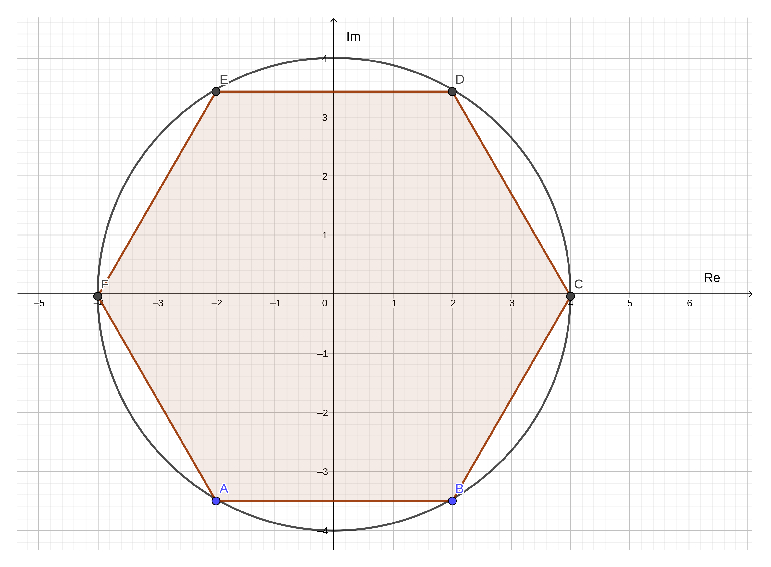
\includegraphics[scale=0.5]{geogebra-export_1.eps}
	\end{figure}

\item Na figura, $P1, P2 \textrm{ e } P3$ são os afixos dos números complexos $z_1, z_2 \textrm{ e } z_3$ , respectivamente. Determine a forma polar de $z_1, z_2 \textrm{ e de } z_3$
	\begin{figure}[h]
	\centering
	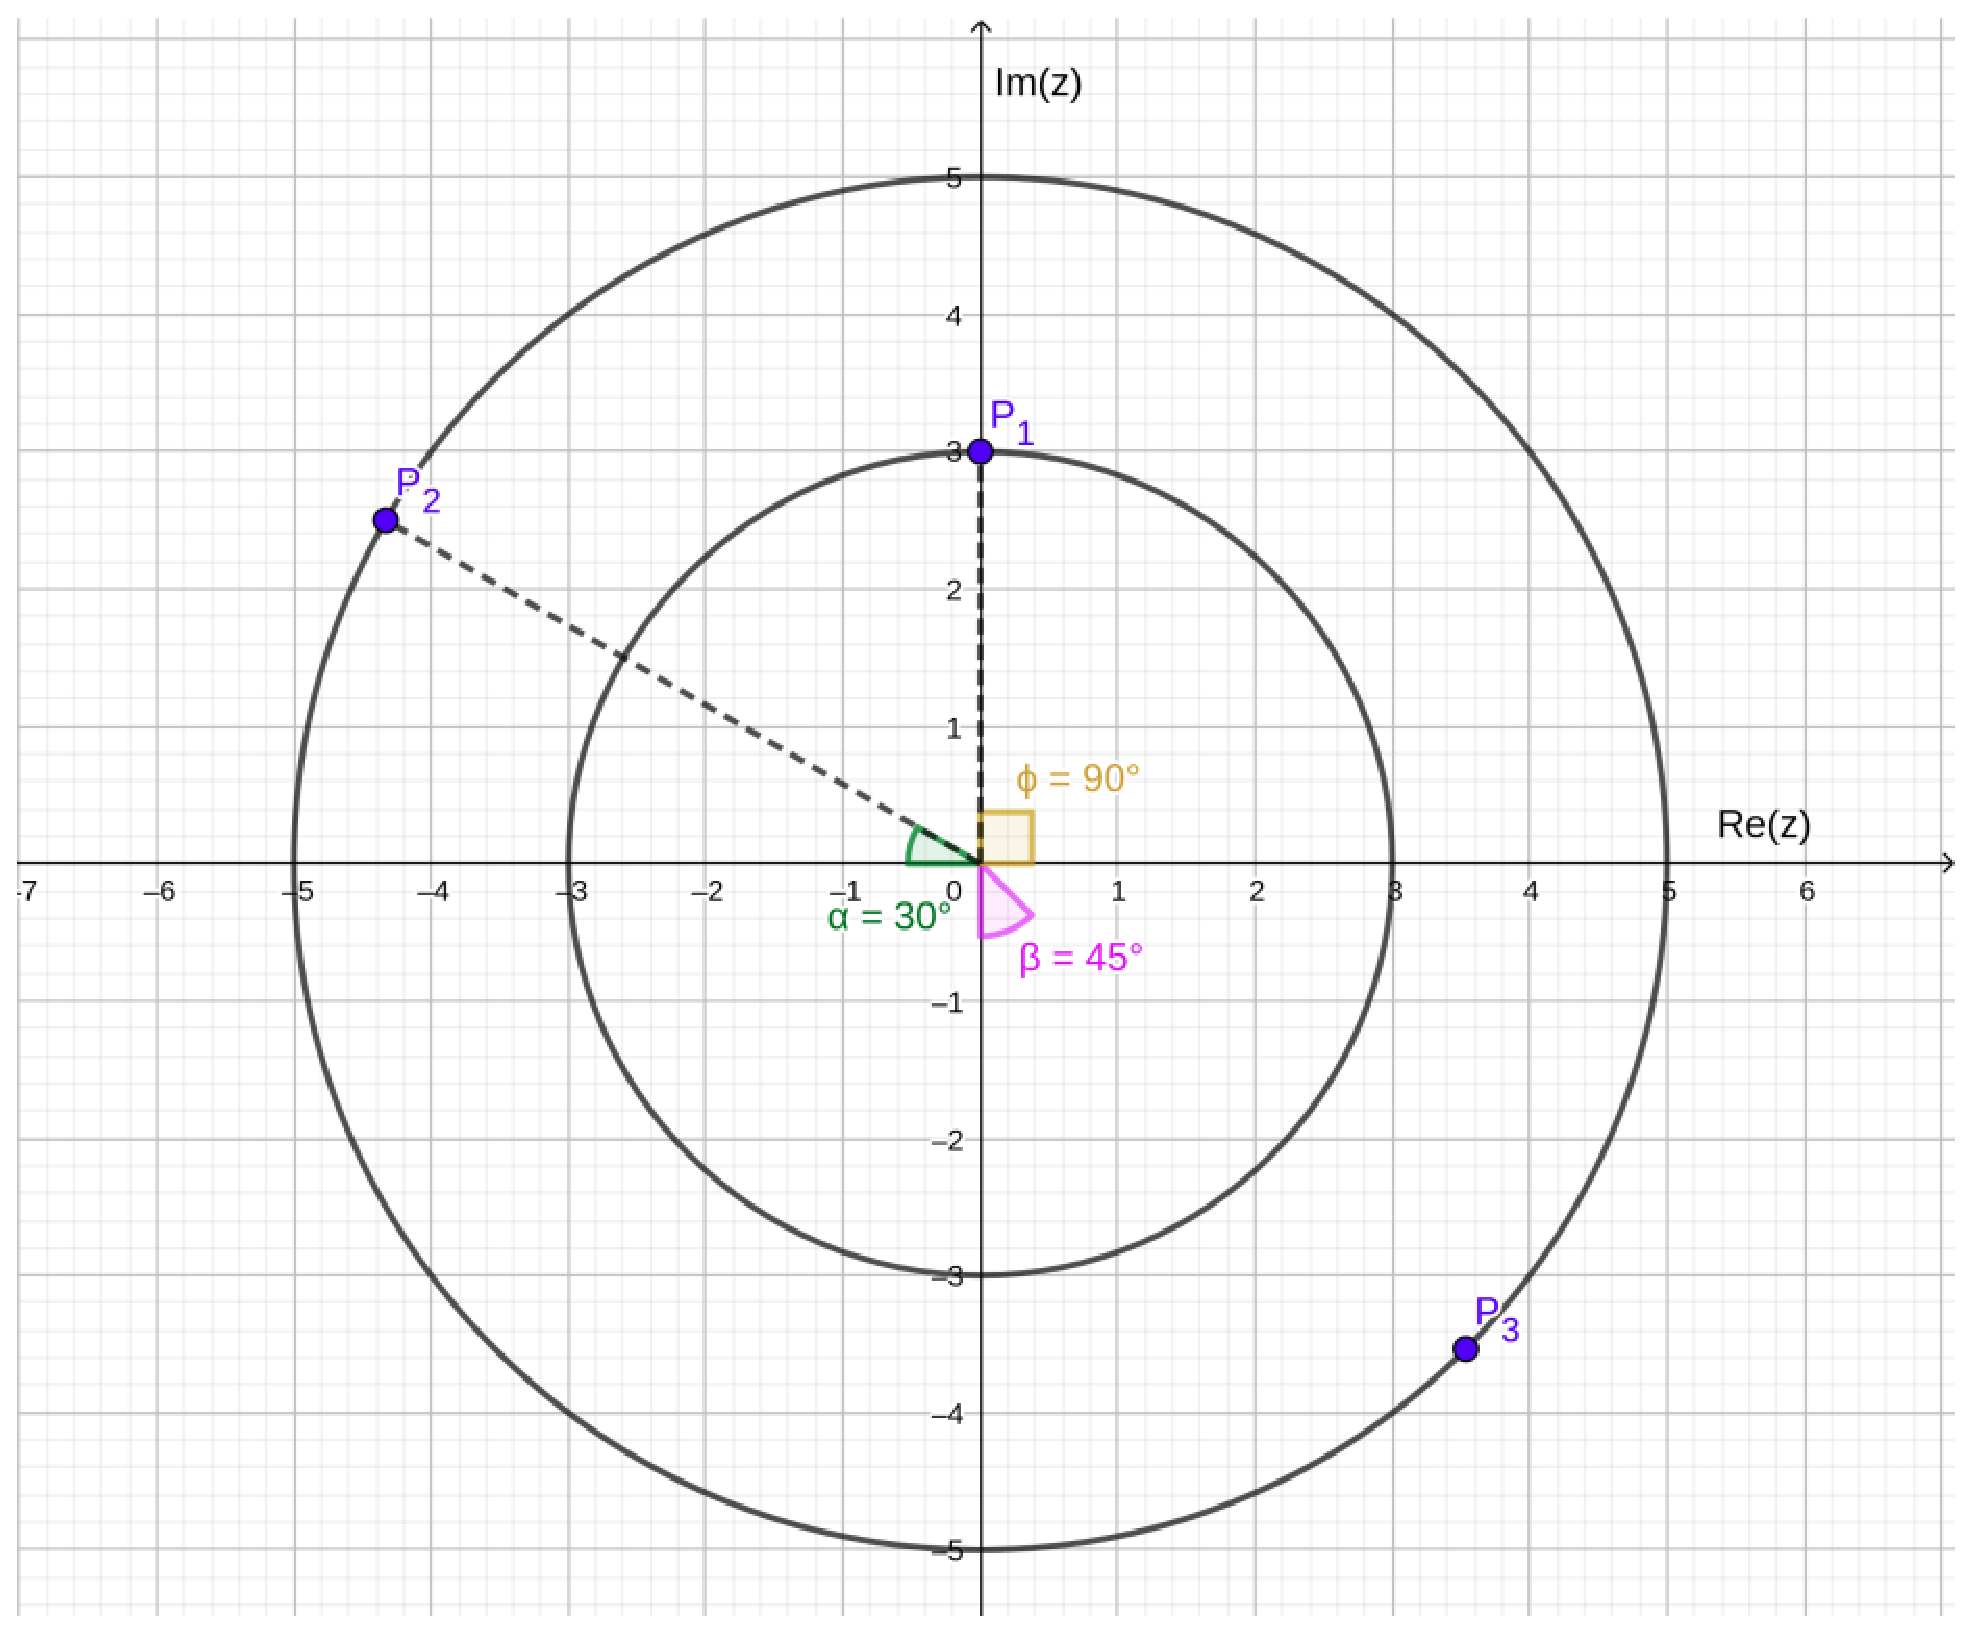
\includegraphics[scale=0.2]{geogebra_2.eps}
	\end{figure}

\item O polígono $ABCDE$ da figura é um pentágono regular inscrito no círculo unitário de centro na origem. Determine as coordenadas polares do vértice A.
	\begin{figure}[!h]
	\centering
	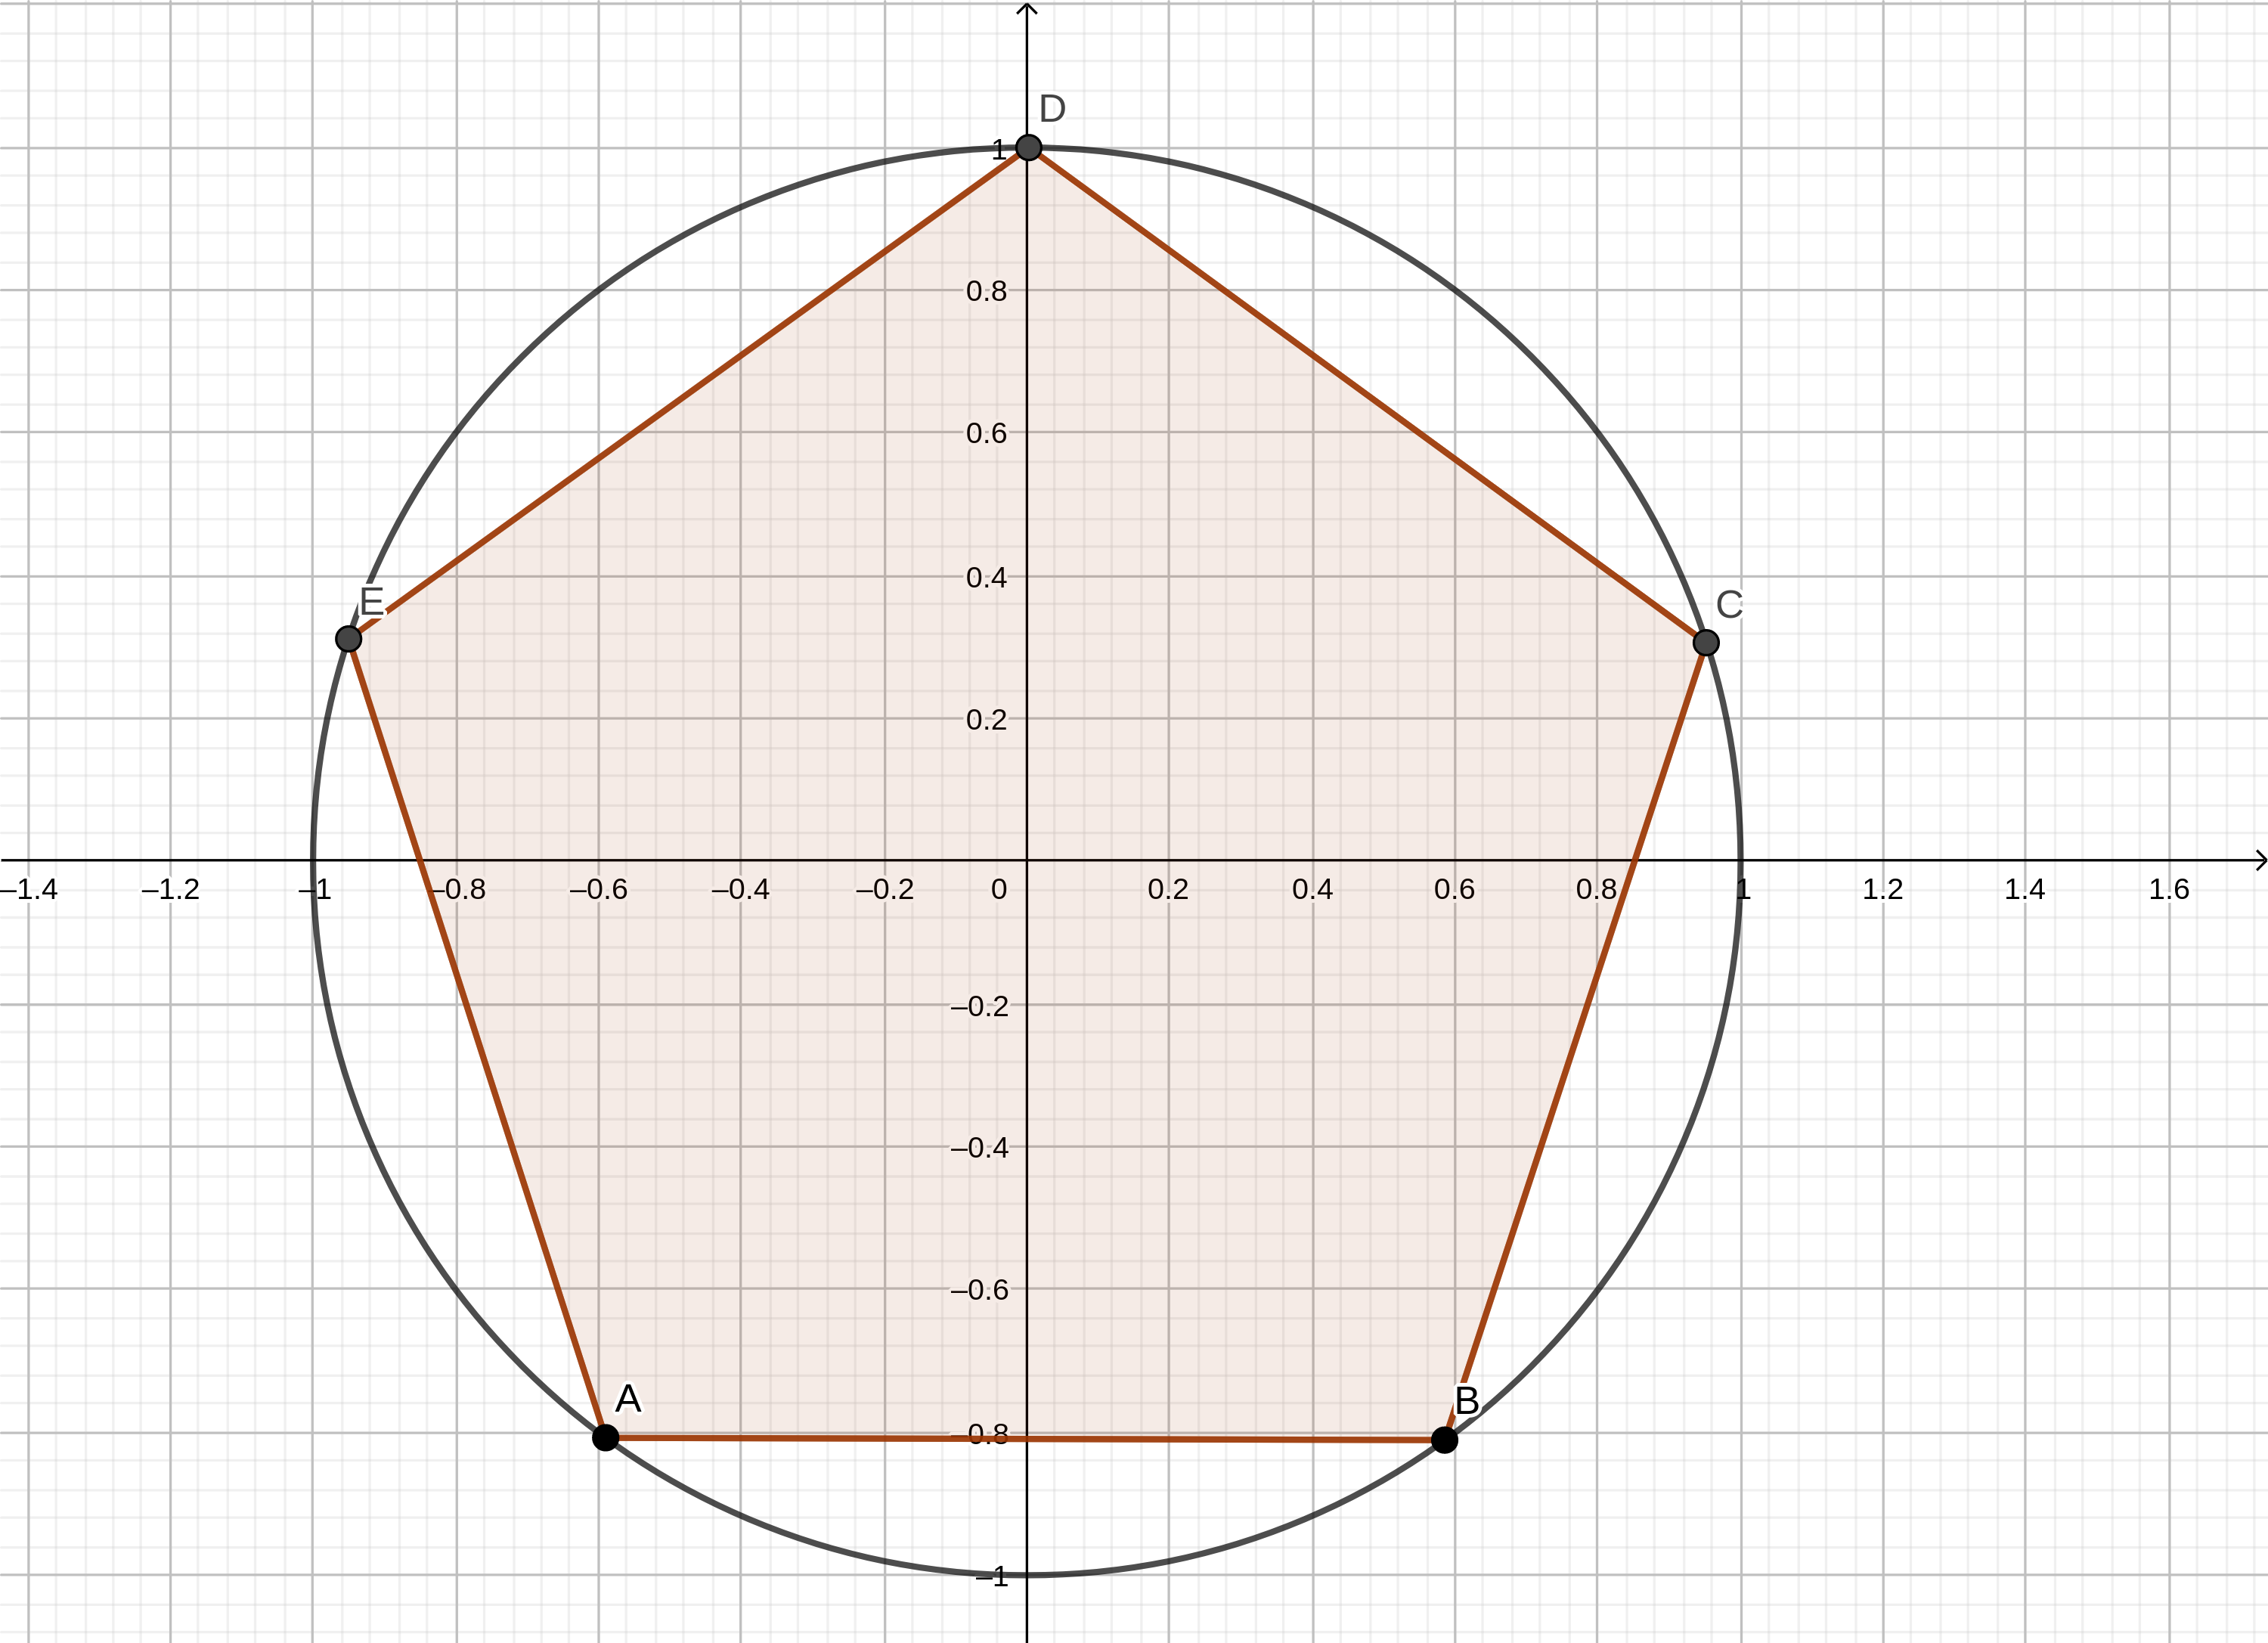
\includegraphics[scale=2.3]{geogebra_3.eps}
	\end{figure}

\item Determine o lugar geométrico do conjunto de afixos de números complexos que possuem o mesmo módulo. Justifique sua resposta.	

\item Conhecendo um número complexo na sua forma polar, como posso escrever a forma polar do seu inverso multiplicativo $z^{-1}$? E do seu conjugado $\overline{z}$?

\item \textbf{Desafio 4:} Dado $z = 7\cdot(cos(\dfrac{\pi}{4}) + i\cdot sin(\dfrac{\pi}{4}))$, descubra os valores de $n \in \mathbb{N}$ para que:
	\begin{enumerate}
	\item $z^n$ seja um número imaginário puro
	\item $z^n$ seja um número real
	
	Dica: Represente $z$ no plano complexo.
	\end{enumerate}

\item \textbf {Desafio 5:} Determine as coordenadas do ponto $P'$, obtido ao se rotacionar o ponto $ P(4\sqrt{2} , 4\sqrt{2})$  em torno da origem, em um ângulo de $225^{\circ}$, no sentido:
	\begin{enumerate}
	\item anti-horário
	\item horário
	\end{enumerate}
	
\item \textbf{Desafio 6:}  No plano complexo, considere a curva $\beta$ descrita pelos pontos 

$z = (1 + cos\theta \cdot (cos(\theta) + isen(\theta))$, para $\theta \in [-\pi, \pi]$ e julgue os seguintes itens.
	\begin{enumerate}
	\item $|z| \leq 2$
	\item Se $z$ é um número real e $z \in \beta$, então $z = 0$
	\item Se $z \in \beta$, então o conjugado de $z$ também pertence a $\beta$
	\end{enumerate}


%%%%%%%%%%%%%%%%%%%%%%%%%%%%%%%%%%%%%%%%%%%%%%%%%%%%%%%%%%%%%%%%%%%%%%%%%%%%%%%%%%%%%%%%%%%%%%%%%%%%%%%%%%%%%

\begin{center}
	\textbf{Potenciação e radiciação de complexos (ou \textit{fórmulas de De Moivre})}
	\\
\end{center}


\item Dado $z = 4\cdot(cos15^{\circ} + i\cdot sin15^{\circ})$, calcule $z^{10}$.

\item Encontre a forma trigonomética de $z = i^{21}\cdot i^{22}\cdot i^{23} \ldots \, i^{29}$. 

\item Dado $z = 2\cdot(cos30^{\circ} + i\cdot sin30^{\circ})$, obtenha a forma retangular de
	\begin{enumerate}
	\item $z^3$
	\item $z^6$
	\item $z^{10}$
	\end{enumerate}
	
\item Sabendo que $z = -1 + \sqrt{3}i$, calcule $z^{6}$, $z^{16}$ e $z^{101}$ e expresse os resultados nas forma polar e algébrica.


\item Dado $z = \sqrt{3} - i$, obtenha $z^6$:
	\begin{enumerate}
	\item sem o uso da fórmula de De Moivre
	\item por meio da fórmula de De Moivre
	\end{enumerate}

\item Calcule:
	\begin{enumerate}
	\item $(-\sqrt{6} -i\sqrt{2})^{13}$
	\item $(\dfrac{1}{5} + \dfrac{1}{5}i)^{101}$
	\item $(-4 + 4i\sqrt{3})^{-6}$
	\end{enumerate}

\item Determine as raízes quadradas dos números complexos seguintes:
	\begin{enumerate}
	\item $i$
	\item $-3$
	\item $-\dfrac{1}{4}$
	\\
	\\
	\end{enumerate}

\item Calcular:
	\begin{enumerate}
	\item $\sqrt[3]{-2+2i\sqrt{3}}$
	\item $\sqrt[4]{-5 -5i}$
	\item $\sqrt{4\sqrt{3} - 4i}$
	\end{enumerate}

\item Interprete, geometricamente, o que representam as duas fórmulas de De Moivre.

\item Dado o complexo $z = 4i$, determine:
	\begin{enumerate}
	\item as raízes quadradas de $z$ e as representações no plano de Argand-Gauss.
	\item a distância entre essas duas raízes.
	\end{enumerate}

\item Sabendo que o ponto $A(-1,0)$ é a imagem de uma das raízes sextas de um número complexo $z$ (isto é, $\sqrt[6]{z}$), determine:
	\begin{enumerate}
	\item $z$
	\item as formas algébrica e polar de cada uma das raízes sextas de $z$.
	\end{enumerate}

\item Um matemático, observando um vitral com o desenho de um polígono inscrito em um círculo, verificou que os vértices desse polígono poderiam ser representados pelas raízes cúbicas complexas do número 8. Qual é a área do polígono observado pelo matemático?


\item \textbf{Desafio 7:} Tendo $i$ como a unidade imaginária, sabemos que $i^2 = -1$. Sendo assim
	\begin{enumerate}
	\item Calcule os valores de $i^3$, $i^4$, $i^5$ e $i^6$.
	\item Calcule o valor de $i^{2019}$.
	\item Encontre uma expressão que relacione um caso genérico de $i^n \, | \, n \in \mathbb{N}$. Reflita sobre o significado da expressão e tente explicá-lo.
	\end{enumerate}

\item \textbf{Desafio 8:} Tendo $i$ como a unidade imaginária, sabemos, por definição, que $i^2 = -1$. Todavia, é comum algumas pessoas apresentarem uma definição da unidade imaginária como sendo $i = \sqrt{-1}$.
	\begin{enumerate}
	\item Escreva o valor de $i$ na forma polar e calcule o valor de $i^2$. 
	\item Escreva $-1$ na forma polar e calcule $\sqrt{-1}$.
	\item Qual das duas definições parece ser a mais apropriada? Justifique sua resposta.
	\end{enumerate}

\item \textbf{Desafio 9:} Uma forma alternativa de escrever os números complexos é usando uma terceira representação: a chamada \textit{forma exponencial}. Ela consiste em usar a identidade de Euler (a qual eu não demonstrarei):
	$$ |z|\cdot ( cos(\theta) + i\cdot sin(\theta) ) = |z|\cdot e^{\theta\cdot i} ,$$
	
	onde $\theta$ é o argumento principal e $|z|$ é o módulo do complexo, já conhecidos nosso.
	
Como exemplo, podemos escrever $i = e^{ 90^{\circ} \cdot i} $, já que seu módulo é $1$ e seu argumento é $90^{\circ}$.

É mais comum, no entanto, escrevermos os argumentos em \textit{radianos}. Quando isso acontece, podemos escrever, já que $90^{\circ} = \dfrac{\pi}{2}$, 

$$i = e^{ 90^{\circ} \cdot i} = e^{\frac{\pi}{2} \cdot i} .$$

A forma mais conhecida é escrevermos 

$$e^{\pi \cdot i} = -1,$$

tendo em vista que $|-1| = 1$ e que o seu argumento vale $\pi \; ( \, = 180^{\circ}).$ Se você parar pra pensar, a equação é meio maluca... Mistura $\pi$, número de euler, unidade imaginária... uma bagunça, não? Mas talvez essa seja sua beleza, afinal.

	\begin{enumerate}
	
	\item Teste se você entendeu esse conceito. Passe para a forma exponencial (com os argumentos em radianos) os números
		\begin{enumerate}
		\item $-i$
		\item $2i$
		\item $3$
		\item $7\cdot cis(45^{\circ})$
		\item $4 + 4i$
		\end{enumerate}
		
	\item Mostre que as propriedades de multiplicação e divisão de complexos na forma polar, bem como a potenciação e radiciação, funcionam para esta forma também. Ao usar a forma exponencial, seu uso parece mais simples ou mais complicado que da forma trigonométrica? 
	
	\item Calcule o valor de $i^i$. Esse número é puramente real, puramente imaginário ou ele tem ambas as partes?
	 Se necessário, use $e^{-\dfrac{\pi}{2}} = 4,81.$
	 Dica: pode ser útil relembrar que $ln(x^n) = n\cdot ln(x).$			
	
	\end{enumerate}

\item \textbf{Desafio 10:} Como introdução ao próximo assunto, segue o desafio.
	\begin{enumerate}
	\item Calcule as raízes da função $f: \mathbb{C} \longrightarrow \mathbb{C} \, | \, f(x) = x^2 -5x + 6$. Essas raízes possuem alguma semelhança? Se sim, qual?
	\item Calcule as raízes da função $g: \mathbb{C} \longrightarrow \mathbb{C} \, | \, g(x) = x^2 + 1$. Essas raízes possuem alguma semelhança? Se sim, qual?
	\item Calcule as raízes da função $z: \mathbb{C} \longrightarrow \mathbb{C} \, | \, z(x) = x^2 + 3x + 12$. Essas raízes possuem alguma semelhança? Se sim, qual?
	\item Compare as semelhanças e as diferenças que você encontrou nos três exemplos acima. Reflita um pouco e responda: foi mera coincidência? Ou será que existe algo mais interessantes por trás...?
	\item O que significa, geometricamente, uma função de variáveis complexas?
	\end{enumerate}















\end{enumerate}




\end{document}